\documentclass{article}

% Required packages
\usepackage{amssymb}
\usepackage{amsmath}
\usepackage{graphicx}
\usepackage{geometry}
\usepackage{tikz}
\usepackage{array}
\usepackage{booktabs}
\usepackage{enumitem}
\usepackage{listings}
\usepackage{xcolor}
\usepackage{fancyhdr}
\usepackage{float}
\usepackage{subcaption}
\usepackage{comment}

% Set page geometry
\geometry{a4paper, margin=1in}

% Configure listings for Python
\lstset{
  language=Python,
  basicstyle=\ttfamily\footnotesize,
  numbers=left,
  numberstyle=\tiny\color{gray},
  frame=single,
  breaklines=true,
  breakatwhitespace=true,
  captionpos=b,
  tabsize=4,
  showspaces=false,
  showstringspaces=false,
  showtabs=false,
  commentstyle=\color{gray}\textit,
  keywordstyle=\color{blue}\bfseries,
  stringstyle=\color{red}
}

\begin{document}

\pagestyle{fancy}
\chead{DSC 255: Machine Learning Fundamentals (Spring 2025)}
\lhead{Homework 9}
\rhead{Randall Rogers}

%------------------
% Solution for (a)
%------------------
\subsection*{Solution 1 (a): Linear Classifiers}
\noindent\rule{\textwidth}{0.4pt}

\subsubsection*{Step 1: Nature of Linear Classifier Boundaries}
\parbox{\textwidth}{
Linear classifiers, by definition, learn a decision boundary that is linear in the feature space. For a feature vector $\mathbf{x}$, this boundary is represented by an equation of the form:
$$ \mathbf{w}^T\mathbf{x} + b = 0 $$
where $\mathbf{w}$ is the weight vector and $b$ is the bias term. This equation defines a hyperplane that divides the feature space into two half-spaces.
}

\subsubsection*{Step 2: Limitation in Expressiveness}
\parbox{\textwidth}{
A single hyperplane can only separate data that is linearly separable. It cannot capture non-linear relationships or create complex, disjoint decision regions. For instance, a linear classifier cannot solve the XOR problem, where data points are arranged in a non-linearly separable pattern. Decision trees, on the other hand, can create multiple axis-aligned splits to isolate regions corresponding to the XOR logic.
}

\subsubsection*{\normalfont{$\therefore$ Conclusion for Linear Classifiers}}
\parbox{\textwidth}{
Linear classifiers are not as expressive as decision trees and cannot represent any arbitrary decision boundary. Their expressive power is limited to linear separations.
}

\noindent\rule{\textwidth}{0.4pt}

\newpage

%------------------
% Solution for (b)
%------------------
\subsection*{Solution 1 (b): Support Vector Machines with a Quadratic Kernel}
\noindent\rule{\textwidth}{0.4pt}

\subsubsection*{Step 1: Nature of SVM Boundaries with Quadratic Kernel}
\parbox{\textwidth}{
Support Vector Machines (SVMs) with a quadratic kernel, $K(\mathbf{x}_i, \mathbf{x}_j) = (\gamma \mathbf{x}_i^T \mathbf{x}_j + r)^d$ with $d=2$, implicitly map the input features into a higher-dimensional space where a linear separation is performed. When projected back to the original input space, this linear separation in the higher-dimensional space corresponds to a non-linear, specifically quadratic, decision boundary. The decision function takes the form:
$$ f(\mathbf{x}) = \sum_{i \in SV} \alpha_i y_i (\gamma \mathbf{x}_i^T \mathbf{x} + r)^2 + b = 0 $$
This equation describes a quadratic surface (e.g., ellipses, parabolas, hyperbolas).
}

\subsubsection*{Step 2: Limitation in Expressiveness}
\parbox{\textwidth}{
While a quadratic boundary is more flexible than a linear one and can capture more complex relationships, it is still restricted to a specific polynomial form (second-degree). It cannot represent all possible decision boundaries, especially those with highly irregular shapes, multiple disjoint regions not separable by a single quadratic function, or boundaries requiring higher-order polynomial terms or other non-polynomial forms that a decision tree can approximate through fine-grained partitioning.
}

\subsubsection*{\normalfont{$\therefore$ Conclusion for SVMs with Quadratic Kernel}}
\parbox{\textwidth}{
SVMs with a quadratic kernel are more expressive than linear classifiers but are not as universally expressive as decision trees. They cannot represent *any* decision boundary, being limited to quadratic forms.
}

\noindent\rule{\textwidth}{0.4pt}

\newpage

%------------------
% Solution for (c)
%------------------
\subsection*{Solution 1 (c): Nearest Neighbor Classifiers}
\noindent\rule{\textwidth}{0.4pt}

\subsubsection*{Step 1: Nature of Nearest Neighbor Boundaries}
\parbox{\textwidth}{
Nearest neighbor classifiers, such as k-Nearest Neighbors (k-NN), classify a new data point based on the majority class of its $k$ closest neighbors in the training dataset. The decision boundary is implicitly defined by the relative positions of the training samples. For a 1-Nearest Neighbor (1-NN) classifier, the decision boundary is precisely the Voronoi tessellation of the feature space, where each cell (associated with a training point) contains all points closer to that training point than to any other. The boundaries between cells are piecewise linear (segments of hyperplanes that are perpendicular bisectors between pairs of points from different classes).
}

\subsubsection*{Step 2: High Expressiveness}
\parbox{\textwidth}{
As the number of training samples $N \to \infty$, a 1-NN classifier can approximate any arbitrarily complex decision boundary. The piecewise linear segments of the Voronoi boundaries can form intricate and highly non-linear shapes. With a sufficient density of training points, these local, linear segments can collectively represent virtually any boundary, no matter how convoluted. For $k > 1$, the boundaries tend to be smoother but still retain high flexibility. Cover and Hart (1967) showed that the asymptotic error rate of the 1-NN rule is bounded by twice the Bayes error rate, indicating its strong learning capability.
}

\subsubsection*{\normalfont{$\therefore$ Conclusion for Nearest Neighbor Classifiers}}
\parbox{\textwidth}{
Nearest neighbor classifiers (especially 1-NN with a sufficient number of diverse training samples) are highly expressive and can represent (or approximate arbitrarily well) any decision boundary, similar in expressive power to decision trees.
}

\noindent\rule{\textwidth}{0.4pt}

\newpage

%------------------
% Solution for (d)
%------------------
\subsection*{Solution 1 (d): Classifiers based on Gaussian Generative Models}
\noindent\rule{\textwidth}{0.4pt}

\subsubsection*{Step 1: Nature of Boundaries from Gaussian Generative Models}
\parbox{\textwidth}{
Classifiers based on Gaussian generative models assume that the class-conditional probability densities $p(\mathbf{x}|C_k)$ follow a Gaussian distribution: $\mathcal{N}(\mathbf{x} | \boldsymbol{\mu}_k, \boldsymbol{\Sigma}_k)$. The decision boundary is derived from comparing posterior probabilities $P(C_k|\mathbf{x})$.
\begin{itemize}
    \item \textbf{Linear Discriminant Analysis (LDA):} Assumes all classes share the same covariance matrix ($\boldsymbol{\Sigma}_k = \boldsymbol{\Sigma}$ for all $k$). This leads to decision boundaries that are linear functions of $\mathbf{x}$.
    \item \textbf{Quadratic Discriminant Analysis (QDA):} Allows each class $C_k$ to have its own covariance matrix $\boldsymbol{\Sigma}_k$. This results in decision boundaries that are quadratic functions of $\mathbf{x}$.
\end{itemize}
}

\subsubsection*{Step 2: Limitation in Expressiveness (for LDA/QDA)}
\parbox{\textwidth}{
\begin{itemize}
    \item LDA, by producing linear boundaries, shares the same limitations as general linear classifiers: it cannot model non-linear relationships.
    \item QDA, by producing quadratic boundaries, is more flexible than LDA but is still restricted to quadratic forms. It cannot model decision boundaries that are more complex than what can be described by a second-degree polynomial.
\end{itemize}
If one were to consider Gaussian Mixture Models (GMMs) to model each $p(\mathbf{x}|C_k)$, then with a sufficient number of Gaussian components, GMMs can approximate any continuous density. Consequently, a Bayes classifier using GMMs could approximate any decision boundary. However, the term "classifiers based on Gaussian generative models" often refers to LDA or QDA in simpler contexts unless GMMs are explicitly specified. Assuming the standard LDA/QDA interpretation:
}

\subsubsection*{\normalfont{$\therefore$ Conclusion for Gaussian Generative Models (LDA/QDA)}}
\parbox{\textwidth}{
Standard classifiers based on Gaussian generative models, such as LDA and QDA, are limited to linear or quadratic decision boundaries, respectively. Therefore, they are not as universally expressive as decision trees and cannot represent any arbitrary decision boundary. (The expressiveness increases significantly if using Gaussian Mixture Models with many components, but this is typically considered a more advanced case.)
}

\noindent\rule{\textwidth}{0.4pt}

\newpage

%------------------
% Solution
%------------------
\subsection*{Solution 2}
\noindent\rule{\textwidth}{0.4pt}

\subsubsection*{Step 1: Number of Ways to Choose a Feature}
\parbox{\textwidth}{
The dataset has $d$ dimensions, which means there are $d$ features available. When selecting a feature to split on, we must choose one of these $d$ features. (\textit{i.e. Number of choices for the feature = $d$.})
%\begin{itemize}
%    \item Number of choices for the feature = $d$.
%\end{itemize}
}

\subsubsection*{Step 2: Effective Number of Splits for a Chosen Feature}
\parbox{\textwidth}{
Once a feature is chosen, we need to determine a split value along that feature. We are considering axis-aligned splits.
\begin{itemize}
    \item \textbf{Continuous Features:} For a continuous feature, potential split points are typically considered between the unique sorted values of that feature present in the $n$ data points at the current node. If we have $n$ data points, let their values for the chosen feature be $x_1, x_2, \ldots, x_n$. After sorting these values as $x_{(1)} \le x_{(2)} \le \ldots \le x_{(n)}$, the potential split points are usually taken as midpoints: $\frac{x_{(i)} + x_{(i+1)}}{2}$ for $i = 1, \ldots, n-1$.
    \item If all $n$ values $x_{(i)}$ are distinct, there are $n-1$ such unique midpoints, and thus $n-1$ possible splits.
    \item If some feature values are repeated, let $u$ be the number of unique sorted values for that feature among the $n$ points ($u \le n$). Then, there are $u-1$ distinct split points to consider.
    \item Since the question asks for a "rough" estimate, and $u-1 \le n-1$, we can consider the maximum number of splits for a feature to be $n-1$. This occurs when all data points have distinct values for that feature.
    \item \textbf{Categorical Features:} If the feature were categorical (though the phrasing "split value along that feature" leans towards continuous), the number of splits would depend on the number of categories and the type of split (e.g., one-vs-rest, or partitioning subsets of categories). For a feature with $k$ unordered categories, there are $2^{k-1}-1$ possible binary splits. For $k$ ordered categories, there are $k-1$ splits. However, the context of "split value" usually implies continuous or ordered data. We will assume continuous features for this "rough" estimate based on the phrasing.
\end{itemize}
So, for a given feature (assuming it's continuous or ordinal), there are at most $n-1$ effective split points to evaluate.
}

\subsubsection*{Step 3: Total Number of Possible Splits to Try}
\parbox{\textwidth}{
To find the total number of possibilities to try out at the top node, we multiply the number of ways to choose a feature by the (maximum) number of effective splits for a feature:
$$ \text{Total Possibilities} = (\text{Number of features}) \times (\text{Max. splits per feature}) $$
$$ \text{Total Possibilities} \approx d \times (n-1) $$
This is a common upper bound used for complexity analysis.
\textbf{Key Assumptions for this estimate:}
\begin{itemize}
    \item We are considering axis-aligned splits.
    \item Features are primarily continuous or ordinal, where splits are defined between sorted values.
    \item For each such feature, there are at most $n-1$ distinct split points among $n$ data points.
    \item We check every feature and every possible split point for each feature.
\end{itemize}
}

\subsubsection*{\normalfont{$\therefore$ Conclusion Statement}}
\parbox{\textwidth}{
Roughly, we need to try out $O(d \cdot n)$ possibilities for splits at the top node of the tree. More precisely, it's approximately $d \times (n-1)$ potential splits.
}

\noindent\rule{\textwidth}{0.4pt}

\newpage

%------------------
% Solution
%------------------
\subsection*{Solution 3}
\noindent\rule{\textwidth}{0.4pt}

\subsubsection*{Step 1: Identify the fraction $p$}
\parbox{\textwidth}{
The problem states that a node has 20\% of points with one label and 80\% with the other label. The Gini impurity formula for two labels is given as $2p(1-p)$, where $p$ is the fraction of one label.

We can choose either fraction for $p$. Let's set $p$ to be the fraction of the first label:
$$ p = 20\% = 0.20 $$
Consequently, the fraction of the other label is $1-p$:
$$ 1-p = 1 - 0.20 = 0.80 $$
This matches the given 80\%. (Alternatively, if we chose $p=0.80$, then $1-p=0.20$, and the formula $2p(1-p)$ would yield the same result due to symmetry.)
}

\subsubsection*{Step 2: Calculate the Gini Impurity Index}
\parbox{\textwidth}{
Now we substitute the value of $p$ into the Gini impurity formula:
$$ \text{Gini Impurity} = 2 \cdot p \cdot (1-p) $$
Plugging in $p = 0.20$:
$$ \text{Gini Impurity} = 2 \cdot (0.20) \cdot (1 - 0.20) $$
$$ \text{Gini Impurity} = 2 \cdot (0.20) \cdot (0.80) $$
$$ \text{Gini Impurity} = 0.40 \cdot (0.80) $$
$$ \text{Gini Impurity} = 0.32 $$
}

\subsubsection*{\normalfont{$\therefore$ Conclusion Statement}}
\parbox{\textwidth}{
The Gini impurity index for a node in which 20\% of the points have one label and 80\% have the other label is 0.32.
}

\noindent\rule{\textwidth}{0.4pt}

\newpage

%------------------
% Solution for (a) - Decision Trees
%------------------
\subsection*{Solution 4 (a): Decision Trees}
\noindent\rule{\textwidth}{0.4pt}

\subsubsection*{Step 1: Weighted Class Proportions}
\parbox{\textwidth}{
To incorporate weights $\lambda_i$ into decision trees, we modify how we calculate the proportion of points belonging to each class at a given node. Let $S$ be the set of indices of data points at a particular node. Let $S_k \subseteq S$ be the set of indices of data points at that node belonging to class $k$.

The weighted proportion $p_k$ for class $k$ at this node is calculated as the sum of weights of points in class $k$ divided by the total sum of weights of all points at the node:
$$ p_k = \frac{\sum_{i \in S_k} \lambda_i}{\sum_{j \in S} \lambda_j} $$
These weighted proportions $\sum_{k} p_k = 1$ are then used in the impurity measures.
}

\subsubsection*{Step 2: Weighted Impurity Measures}
\parbox{\textwidth}{
Once we have the weighted proportions $p_k$, we can compute weighted versions of impurity measures:
\begin{itemize}
    \item \textbf{Weighted Gini Impurity:} The Gini impurity for a node becomes:
    $$ \text{Gini}_{\text{weighted}} = 1 - \sum_{k} p_k^2 = \sum_{k} p_k (1-p_k) $$
    If there are two classes, and $p$ is the weighted proportion of one class, this is $2p(1-p)$ using the weighted $p$.

    \item \textbf{Weighted Entropy:} The entropy for a node becomes:
    $$ \text{Entropy}_{\text{weighted}} = - \sum_{k} p_k \log_2(p_k) $$
    (where $0 \log_2 0$ is taken as 0).
\end{itemize}
The decision tree algorithm then seeks splits that maximize the reduction in these weighted impurity measures. The information gain (or gain ratio) would be calculated using these weighted impurity values.
}

\subsubsection*{Step 3: Other Considerations}
\parbox{\textwidth}{
\begin{itemize}
    \item \textbf{Split Evaluation:} When evaluating a potential split, the weighted impurity of the resulting child nodes is calculated, and the overall quality of the split is a weighted average of these child node impurities, where the weights are the proportion of total weight going to each child.
    \item \textbf{Stopping Criteria:} Stopping criteria like "minimum samples per leaf" should be interpreted as "minimum sum of weights per leaf". For example, a leaf might be considered too small if $\sum_{i \in \text{Leaf}} \lambda_i < \text{min\_weight\_leaf}$.
    \item \textbf{Leaf Node Prediction:} The prediction at a leaf node is typically the majority class based on the sum of weights for each class within that leaf.
\end{itemize}
}

\subsubsection*{\normalfont{$\therefore$ Conclusion for Decision Trees}}
\parbox{\textwidth}{
By redefining class proportions using sums of weights, and subsequently using these weighted proportions in impurity calculations (Gini, Entropy) and stopping criteria, decision trees can effectively handle weighted data without explicit duplication. The core logic of finding the best split remains, but the "count" of data points is replaced by their cumulative weight.
}

\noindent\rule{\textwidth}{0.4pt}

\newpage

%------------------
% Solution for (b) - Gaussian Generative Models
%------------------
\subsection*{Solution 4 (b): Gaussian Generative Models}
\noindent\rule{\textwidth}{0.4pt}

\subsubsection*{Step 1: Weighted Class Priors ($\pi_j$)}
\parbox{\textwidth}{
In a Gaussian generative model, the class prior $\pi_j = P(C_j)$ is typically estimated as the fraction of training samples belonging to class $j$. With weighted data, let $N$ be the total number of data points. Let $I_j$ be the set of indices of data points belonging to class $j$. The weighted class prior $\pi_j$ is the sum of weights of samples in class $j$ divided by the total sum of weights of all samples:
$$ \pi_j = \frac{\sum_{i \in I_j} \lambda_i}{\sum_{m=1}^{N} \lambda_m} $$
}

\subsubsection*{Step 2: Weighted Mean ($\boldsymbol{\mu}_j$)}
\parbox{\textwidth}{
The mean $\boldsymbol{\mu}_j$ for class $j$ is the average of the feature vectors $\mathbf{x}^{(i)}$ belonging to class $j$. For weighted data, this becomes a weighted average:
$$ \boldsymbol{\mu}_j = \frac{\sum_{i \in I_j} \lambda_i \mathbf{x}^{(i)}}{\sum_{i \in I_j} \lambda_i} $$
Each data point $\mathbf{x}^{(i)}$ in class $j$ contributes to the mean proportionally to its weight $\lambda_i$.
}

\subsubsection*{Step 3: Weighted Covariance Matrix ($\boldsymbol{\Sigma}_j$)}
\parbox{\textwidth}{
The covariance matrix $\boldsymbol{\Sigma}_j$ for class $j$ measures the spread and correlation of features for that class. For weighted data, it is estimated as:
$$ \boldsymbol{\Sigma}_j = \frac{\sum_{i \in I_j} \lambda_i (\mathbf{x}^{(i)} - \boldsymbol{\mu}_j)(\mathbf{x}^{(i)} - \boldsymbol{\mu}_j)^T}{\sum_{i \in I_j} \lambda_i} $$
This is for Quadratic Discriminant Analysis (QDA) where each class has its own covariance matrix. For Linear Discriminant Analysis (LDA), a pooled weighted covariance matrix $\boldsymbol{\Sigma}$ would be computed:
$$ \boldsymbol{\Sigma} = \sum_{j=1}^{k} \frac{\sum_{i \in I_j} \lambda_i}{\sum_{m=1}^{N} \lambda_m} \boldsymbol{\Sigma}_j^{\text{class-specific}} = \frac{\sum_{j=1}^{k} \sum_{i \in I_j} \lambda_i (\mathbf{x}^{(i)} - \boldsymbol{\mu}_j)(\mathbf{x}^{(i)} - \boldsymbol{\mu}_j)^T}{\sum_{m=1}^{N} \lambda_m} $$
(Careful with denominators: some formulations use a bias correction like $N_j-1$ or $\sum \lambda_i - 1$; for weighted versions, one might use $\sum_{i \in I_j} \lambda_i$ or a more complex effective sample size if unbiased estimation is critical, but the forms above are common for MLE-like estimates). For simplicity, the denominator $\sum_{i \in I_j} \lambda_i$ is often used for $\boldsymbol{\Sigma}_j$.
}

\subsubsection*{\normalfont{$\therefore$ Conclusion for Gaussian Generative Models}}
\parbox{\textwidth}{
For Gaussian generative models, sample weights $\lambda_i$ are incorporated by using weighted sums to estimate the class priors $\pi_j$, class means $\boldsymbol{\mu}_j$, and class covariance matrices $\boldsymbol{\Sigma}_j$ (or the pooled covariance $\boldsymbol{\Sigma}$). Each parameter estimation becomes a weighted version of its unweighted counterpart.
}

\noindent\rule{\textwidth}{0.4pt}

\newpage

%------------------
% Solution for (c) - Support Vector Machines
%------------------
\subsection*{Solution 4 (c): Support Vector Machines}
\noindent\rule{\textwidth}{0.4pt}

\subsubsection*{Step 1: Standard Soft-Margin SVM Objective}
\parbox{\textwidth}{
The primal objective function for a soft-margin linear SVM is typically:
$$ \min_{\mathbf{w}, b, \boldsymbol{\xi}} \frac{1}{2} \|\mathbf{w}\|^2 + C \sum_{i=1}^{N} \xi_i $$
subject to:
$$ y^{(i)}(\mathbf{w}^T \mathbf{x}^{(i)} + b) \ge 1 - \xi_i, \quad \xi_i \ge 0 \quad \text{for } i=1, \ldots, N $$
Here, $C$ is the regularization parameter that balances margin maximization and misclassification penalty, and $\xi_i$ are slack variables allowing for misclassifications.
}

\subsubsection*{Step 2: Incorporating Weights into the Objective Function}
\parbox{\textwidth}{
To incorporate sample weights $\lambda_i > 0$, we can modify the penalty term for the slack variables. Points with higher weights will incur a larger penalty if they are misclassified or fall within the margin. The objective function becomes:
$$ \min_{\mathbf{w}, b, \boldsymbol{\xi}} \frac{1}{2} \|\mathbf{w}\|^2 + C \sum_{i=1}^{N} \lambda_i \xi_i $$
The constraints remain the same:
$$ y^{(i)}(\mathbf{w}^T \mathbf{x}^{(i)} + b) \ge 1 - \xi_i, \quad \xi_i \ge 0 \quad \text{for } i=1, \ldots, N $$
Effectively, the parameter $C$ is scaled on a per-sample basis to $C_i = C \lambda_i$. This means that the trade-off between maximizing the margin and correctly classifying point $i$ is now influenced by $\lambda_i$. A larger $\lambda_i$ makes it more important to classify point $i$ correctly (or with a smaller $\xi_i$).
}

\subsubsection*{Step 3: Dual Formulation (Conceptual)}
\parbox{\textwidth}{
In the dual formulation, the Lagrange multipliers $\alpha_i$ are typically bounded by $0 \le \alpha_i \le C$. With weighted samples, these bounds would change to $0 \le \alpha_i \le C \lambda_i$. This is how many SVM solvers implement sample weighting.
The dual problem would be:
$$ \max_{\boldsymbol{\alpha}} \sum_{i=1}^N \alpha_i - \frac{1}{2} \sum_{i=1}^N \sum_{j=1}^N \alpha_i \alpha_j y^{(i)} y^{(j)} K(\mathbf{x}^{(i)}, \mathbf{x}^{(j)}) $$
subject to:
$$ \sum_{i=1}^N \alpha_i y^{(i)} = 0 $$
$$ 0 \le \alpha_i \le C \lambda_i \quad \text{for } i=1, \ldots, N $$
where $K(\mathbf{x}^{(i)}, \mathbf{x}^{(j)})$ is the kernel function.
}

\subsubsection*{\normalfont{$\therefore$ Conclusion for Support Vector Machines}}
\parbox{\textwidth}{
For Support Vector Machines, sample weights $\lambda_i$ are incorporated by modifying the objective function to penalize errors on high-weight samples more heavily. This is achieved by multiplying the slack variable $\xi_i$ for each sample $i$ by its weight $\lambda_i$ in the sum of slack penalties, effectively using a per-sample regularization parameter $C_i = C \lambda_i$.
}

\noindent\rule{\textwidth}{0.4pt}

\newpage

%------------------
% Solution for (a)
%------------------
\subsection*{Solution 5 (a): Zero Test Error}
\noindent\rule{\textwidth}{0.4pt}

\subsubsection*{Step 1: Statement Evaluation}
\parbox{\textwidth}{
The statement "Boosting converges to a final classifier with zero test error" is \textbf{False}.
}

\subsubsection*{Step 2: Explanation}
\parbox{\textwidth}{
Boosting algorithms, like AdaBoost, are designed to minimize an objective function related to the \emph{training error}. While AdaBoost has theoretical guarantees about driving the training error towards zero (as discussed in part b), these guarantees do not directly extend to the test error.
\begin{itemize}
    \item \textbf{Overfitting:} If boosting is run for too many iterations, or if the weak learners are too complex (though the premise here is "weak classifiers"), the combined model can overfit the training data. An overfit model performs well on training data but poorly on unseen test data.
    \item \textbf{No Free Lunch:} No learning algorithm can guarantee zero test error on all possible problems. Test error depends on how well the training data represents the true underlying distribution, the complexity of the true concept, and the capacity of the learned model.
    \item \textbf{Margin Theory:} While boosting often exhibits good generalization performance, sometimes attributed to its tendency to increase the margin on training examples, this does not imply zero test error. A large margin is beneficial for generalization but not a guarantee of perfection on unseen data.
\end{itemize}
The condition that the weak learner's error is at most $\tfrac12 - \epsilon$ ensures that boosting can effectively reduce training error, but it doesn't control for the inherent generalization gap between training and test performance.
}

\subsubsection*{\normalfont{$\therefore$ Conclusion for Zero Test Error}}
\parbox{\textwidth}{
Boosting does not guarantee convergence to zero test error. It optimizes performance on the training set, and while it often generalizes well, achieving zero test error is not a guaranteed outcome and is generally unrealistic for non-trivial problems.
}

\noindent\rule{\textwidth}{0.4pt}

\newpage

%------------------
% Solution for (b)
%------------------
\subsection*{Solution 5 (b): Zero Training Error}
\noindent\rule{\textwidth}{0.4pt}

\subsubsection*{Step 1: Statement Evaluation}
\parbox{\textwidth}{
The statement "Boosting converges to a final classifier with zero training error" is \textbf{True} (under the given conditions and assuming enough iterations).
}

\subsubsection*{Step 2: Explanation}
\parbox{\textwidth}{
AdaBoost is designed to minimize an exponential loss function on the training data. The condition that each weak learner $h_t$ has a weighted error $\text{err}_t \le \frac{1}{2} - \epsilon$ (where $\epsilon > 0$) is crucial. This condition ensures that each weak learner performs better than random guessing on the current distribution of weights.
\begin{itemize}
    \item \textbf{Training Error Bound:} AdaBoost has a well-known training error bound. After $T$ rounds of boosting, the training error $E_{\text{train}}$ of the final classifier $H(\mathbf{x}) = \text{sign}(\sum_{t=1}^T \alpha_t h_t(\mathbf{x}))$ is bounded by:
    $$ E_{\text{train}} \le \exp\left(-2 \sum_{t=1}^T \gamma_t^2\right) $$
    where $\gamma_t = \frac{1}{2} - \text{err}_t$ is the "edge" of the weak learner $h_t$. Since $\text{err}_t \le \frac{1}{2} - \epsilon$, it follows that $\gamma_t \ge \epsilon > 0$.
    \item \textbf{Convergence to Zero:} As $T \to \infty$, if $\gamma_t \ge \epsilon$ for all $t$, then $\sum_{t=1}^T \gamma_t^2 \to \infty$. Consequently, $\exp(-2 \sum_{t=1}^T \gamma_t^2) \to 0$.
    This means the training error can be driven arbitrarily close to zero as the number of boosting iterations increases, provided the weak learning condition holds.
    \item \textbf{Exponential Loss:} AdaBoost can be viewed as a stage-wise additive model fitting an exponential loss function. The ability to always find a weak learner better than random guessing allows the algorithm to continuously reduce this loss, which in turn reduces the training misclassification error.
\end{itemize}
}

\subsubsection*{\normalfont{$\therefore$ Conclusion for Zero Training Error}}
\parbox{\textwidth}{
Given that a weak learner with error at most $\tfrac12 - \epsilon$ can always be found, boosting (specifically AdaBoost) is guaranteed to converge to a final classifier with zero training error as the number of iterations increases.
}

\noindent\rule{\textwidth}{0.4pt}

\newpage

%------------------
% Solution for (c)
%------------------
\subsection*{Solution 5 (c): Final Classifier Belongs to Class $\mathcal H$}
\noindent\rule{\textwidth}{0.4pt}

\subsubsection*{Step 1: Statement Evaluation}
\parbox{\textwidth}{
The statement "Boosting's final classifier belongs to class $\mathcal H$" is \textbf{False}.
}

\subsubsection*{Step 2: Explanation}
\parbox{\textwidth}{
The class $\mathcal H$ represents the set of possible \emph{weak} classifiers (e.g., decision stumps, which are decision trees of depth 1). The final classifier produced by boosting, $H(\mathbf{x})$, is a weighted linear combination of these weak classifiers:
$$ H(\mathbf{x}) = \text{sign}\left(\sum_{t=1}^T \alpha_t h_t(\mathbf{x})\right) $$
where $h_t \in \mathcal H$ and $\alpha_t$ are weights assigned to each weak learner.
\begin{itemize}
    \item \textbf{Linear Combination:} The final classifier is formed by summing the outputs of multiple weak learners, each weighted by $\alpha_t$. The decision is then made based on the sign of this sum.
    \item \textbf{Increased Complexity:} This weighted sum is generally a more complex function than any individual weak learner $h_t \in \mathcal H$. For example, if $\mathcal H$ is the class of decision stumps (axis-aligned splits), the final boosted classifier can form a non-linear, non-axis-aligned, and much more intricate decision boundary. It is not itself a decision stump.
    \item \textbf{Closure Property:} The class $\mathcal H$ would need to be closed under weighted linear combinations and the sign operation for $H(\mathbf{x})$ to also be in $\mathcal H$. This is not true for typical classes of weak learners like decision stumps or shallow decision trees.
\end{itemize}
For instance, if $\mathcal{H}$ is the set of decision stumps, each $h_t$ is a very simple classifier. The final $H(\mathbf{x})$ can represent a much more complex decision boundary, far beyond what a single stump can achieve.
}

\subsubsection*{\normalfont{$\therefore$ Conclusion for Final Classifier's Class}}
\parbox{\textwidth}{
Boosting's final classifier is a weighted ensemble of classifiers from $\mathcal H$ and, as such, is generally much more expressive and does not itself belong to the original class of weak learners $\mathcal H$.
}

\noindent\rule{\textwidth}{0.4pt}

\newpage

%------------------
% Solution for (a)
%------------------
\subsection*{Solution 6 (a): The trees can be trained in parallel.}
\noindent\rule{\textwidth}{0.4pt}

\subsubsection*{Step 1: Parallelism in Random Forests}
\parbox{\textwidth}{
In a Random Forest, each decision tree is trained independently of the others. Each tree is built using a different bootstrap sample of the training data and considers a random subset of features at each split. Since the construction of one tree does not depend on the outcome or structure of any other tree, their training processes can be executed simultaneously on multiple CPU cores or even distributed across multiple machines.
}

\subsubsection*{Step 2: Sequential Nature of Boosted Trees}
\parbox{\textwidth}{
Boosted decision trees (like AdaBoost or Gradient Boosting) are built sequentially. Each new tree is trained to correct the errors (or residuals, in the case of gradient boosting) made by the ensemble of previously trained trees. The weights of the training instances are adjusted at each step to emphasize the importance of previously misclassified points. This inherent sequential dependency means that tree $t$ cannot be trained until trees $1, \ldots, t-1$ have been finalized.
}

\subsubsection*{\normalfont{$\therefore$ Conclusion Statement}}
\parbox{\textwidth}{
Yes, the ability to train trees in parallel is a significant benefit of Random Forests over boosted decision trees. This parallelism can lead to substantially faster training times for Random Forests, especially on large datasets and multi-core hardware, whereas boosted trees are constrained by their sequential training process.
}

\noindent\rule{\textwidth}{0.4pt}

\newpage

%------------------
% Solution for (b)
%------------------
\subsection*{Solution 6 (b): Each individual tree is more highly optimized.}
\noindent\rule{\textwidth}{0.4pt}

\subsubsection*{Step 1: Individual Tree Characteristics in Random Forests}
\parbox{\textwidth}{
Individual trees in a Random Forest are typically grown to a large depth (often fully grown, unless parameters like \texttt{max\_depth} or \texttt{min\_samples\_leaf} are set to prune them). They are trained to fit their respective bootstrap samples of the data as well as possible, aiming for low bias on that sample. In this sense, each tree is "optimized" to capture the patterns in the subset of data it sees, subject to the random feature selection at each split. This results in complex individual trees that have low bias but potentially high variance.
}

\subsubsection*{Step 2: Individual Tree Characteristics in Boosted Trees}
\parbox{\textwidth}{
Individual trees in boosting algorithms are intentionally kept "weak" – meaning they are simple and have high bias. Common choices include decision stumps (trees of depth 1) or shallow trees (e.g., depth 2-6). While each weak learner is optimized to best reduce the current weighted error or residuals of the ensemble, its capacity is deliberately limited. The strength of boosting comes from iteratively adding these weak learners, each focusing on the "hard" examples from previous rounds.
}

\subsubsection*{\normalfont{$\therefore$ Conclusion Statement}}
\parbox{\textwidth}{
Yes, if "highly optimized" is interpreted as being more complex and having lower bias on the data it is trained on, then each individual tree in a Random Forest is generally more highly optimized than each individual (weak learner) tree in a boosted decision tree ensemble. Random Forests leverage these individually complex (low-bias, high-variance) trees through bagging to reduce overall variance. This design choice, where individual components are more powerful standalone models, can be seen as a benefit of RF's strategy compared to boosting's reliance on intentionally simple components.
}

\noindent\rule{\textwidth}{0.4pt}

\newpage

%------------------
% Solution for (c)
%------------------
\subsection*{Solution 6 (c): Each individual tree has better accuracy.}
\noindent\rule{\textwidth}{0.4pt}

\subsubsection*{Step 1: Accuracy of Individual Trees in Random Forests}
\parbox{\textwidth}{
As discussed in (b), individual trees in a Random Forest are typically deep and aim for low bias on their bootstrap sample. While they might have high variance and may not generalize perfectly on their own, their accuracy on unseen data (if evaluated independently) is generally moderate to good. They are designed to be reasonably strong learners.
}

\subsubsection*{Step 2: Accuracy of Individual Trees in Boosted Trees}
\parbox{\textwidth}{
Individual trees in boosting ensembles are, by design, weak learners. Their accuracy on the (weighted) training data is only required to be slightly better than random guessing (e.g., error rate $<\!0.5$ for AdaBoost with binary classification). Consequently, their standalone accuracy on unseen data is typically quite low.
}

\subsubsection*{\normalfont{$\therefore$ Conclusion Statement}}
\parbox{\textwidth}{
Yes, each individual tree in a Random Forest generally has better standalone accuracy than each individual tree in a boosted decision tree ensemble. Random Forests rely on averaging these relatively more accurate (though high-variance) base learners to produce a strong final model. This characteristic of employing individually more accurate base models is a feature of RF's design and can be considered a benefit when comparing the nature of the constituent learners to those in boosting.
}

\noindent\rule{\textwidth}{0.4pt}

\newpage


\subsection*{Solution 7 (a)}
\noindent\rule{\textwidth}{0.4pt}\\

\subsubsection*{Sneak Preview at mini-data.txt}

\begin{figure}[H]
  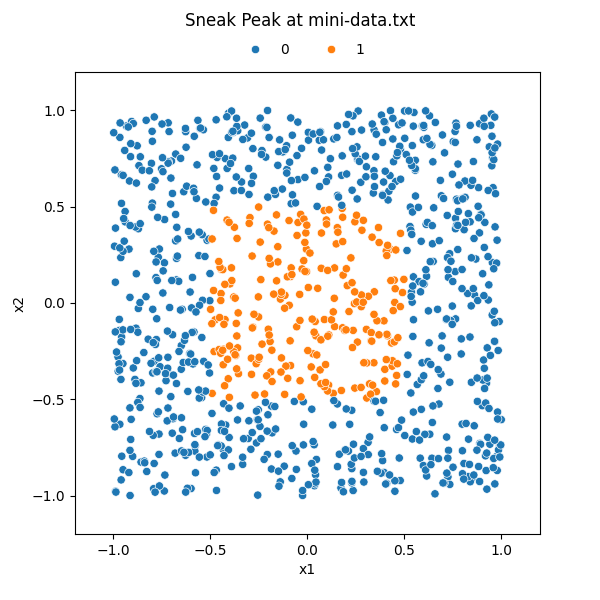
\includegraphics{hw9_q7a.png}
  \caption{Sneak Peak of mini-data.txt, reveals a square doughnut shape.}
\end{figure}

\noindent\rule{\textwidth}{0.4pt}\\

\newpage

\subsection*{Solution 7 (b)}
\noindent\rule{\textwidth}{0.4pt}\\

\subsubsection*{DecisionTreeClassifier: Stop condition}
\begin{table}[h!]               
  \centering                    
  \begin{tabular}{|c|c|c|}
    \hline
    Max depth & Training accuracy & Test accuracy \\ \hline
    1 & 0.50 & 0.49 \\ 
    2 & 0.76 & 0.75 \\ 
    3 & 0.88 & 0.90 \\ 
    4 & 1.00 & 1.00 \\ \hline
  \end{tabular}
  \caption{The stop condition selected was \texttt{max\_depth=4}}   
  \label{tab:depth_accuracy}
\end{table}

\subsubsection*{Python Code}
\begin{lstlisting}
from sklearn.tree import DecisionTreeClassifier
from sklearn.model_selection import train_test_split

x_train, x_test, y_train, y_test = train_test_split(x_data,
                                                    y_data,
                                                    test_size=0.2,
                                                    random_state=42)

def dtc_q7(x_train, x_test, y_train, y_test,n):
    dtc = DecisionTreeClassifier(criterion='log_loss',
                                 max_depth=n,
                                 max_leaf_nodes=n+1,
                                 class_weight='balanced',
                                 min_samples_leaf=int(len(x_train)*0.015),
                                 random_state=42)
    dtc.fit(x_train,y_train)
    print(f"train score(max_depth={n}): {dtc.score(x_train,y_train)}")
    print(f"test score(max_depth={n}): {dtc.score(x_test,y_test)}")

for n in range(1,5):
    dtc_q7(x_train, x_test, y_train, y_test,n)
\end{lstlisting}


\noindent\rule{\textwidth}{0.4pt}\\

\newpage

\subsection*{Solution 7 (c)}
\noindent\rule{\textwidth}{0.4pt}\\

\subsubsection*{Plot}
\begin{figure}[H]
  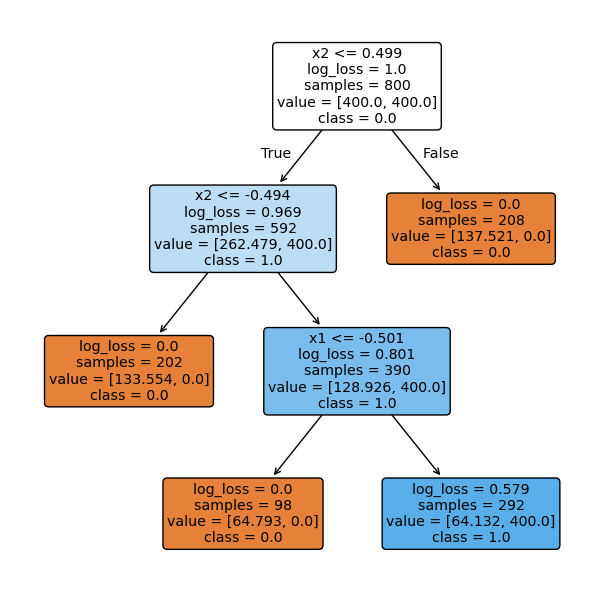
\includegraphics{hw9_q7c.png}
  \caption{Tree plot from the decision tree classifier.}
\end{figure}

\noindent\rule{\textwidth}{0.4pt}\\

\newpage

\subsection*{Solution 7 (d)}
\noindent\rule{\textwidth}{0.4pt}\\
\subsubsection*{Stump Plots}
\begin{center}
  \begin{figure}[H]
    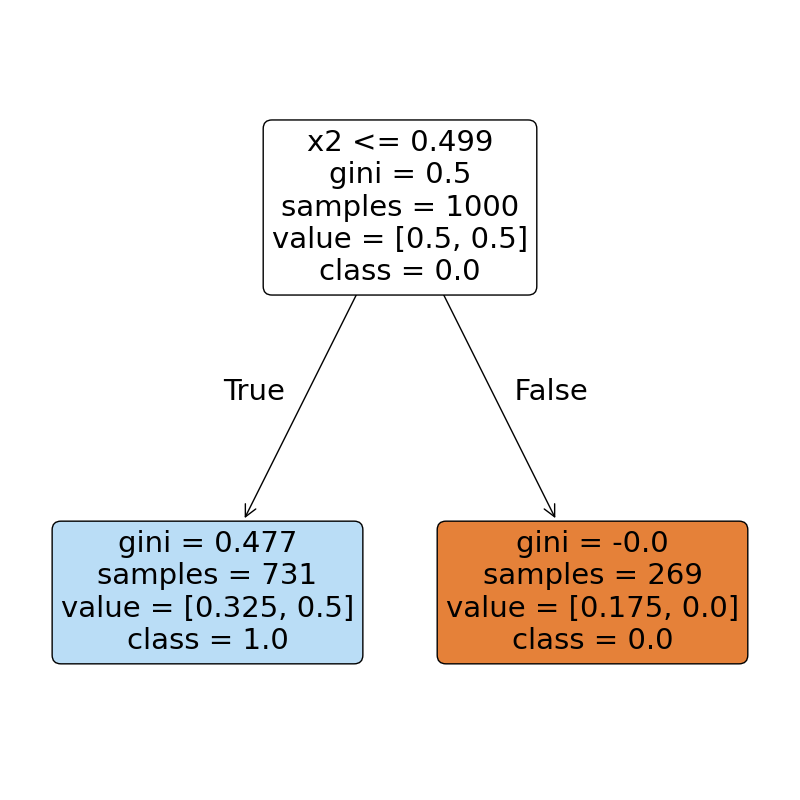
\includegraphics{hw9_q7d_ada_stumps_1.png}
    \caption{Tree plot from the ada boost with one stump}
  \end{figure}
\end{center}

\begin{center}
  \begin{figure}[H]
    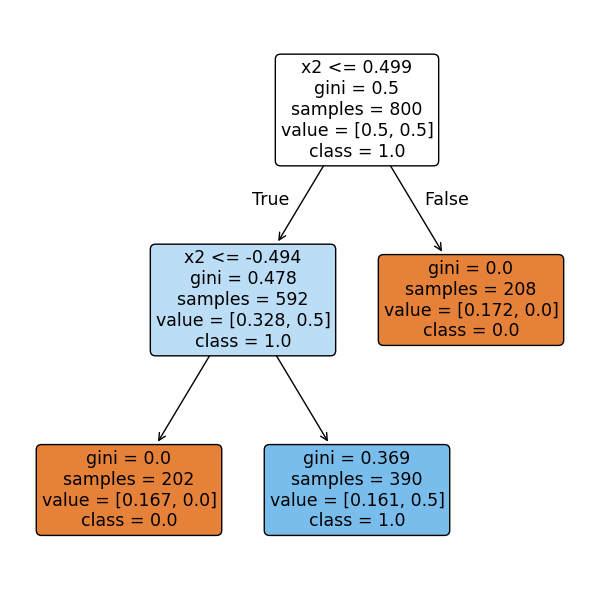
\includegraphics{hw9_q7d_ada_stumps_2.png}
    \caption{Tree plot from the ada boost with two stumps}
  \end{figure}
\end{center}

\begin{center}
  \begin{figure}[H]
    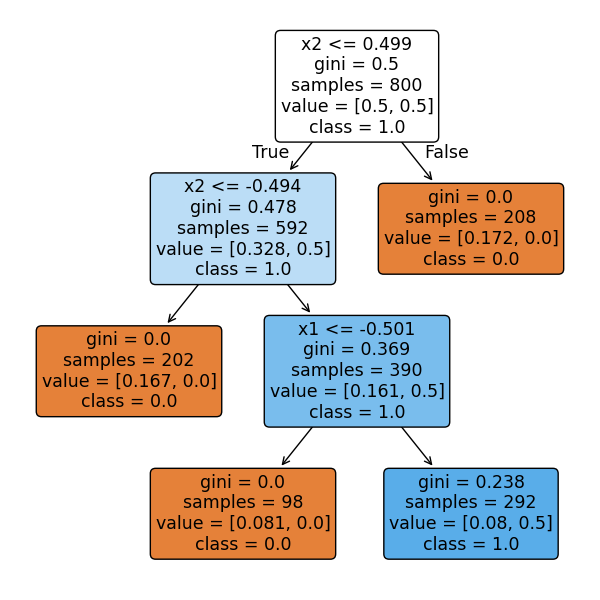
\includegraphics{hw9_q7d_ada_stumps_3.png}
    \caption{Tree plot from the ada boost with three stumps}
  \end{figure}
\end{center}


\noindent\rule{\textwidth}{0.4pt}\\

\newpage

\subsection*{Solution 7 (e)}
\noindent\rule{\textwidth}{0.4pt}\\

\subsubsection*{Ada Boost Training Accuracy}
\begin{table}[h!]               
  \centering                    
  \begin{tabular}{|c|c|}
    \hline
    Stumps & Training accuracy \\ \hline
    1 & 0.50 \\ 
    2 & 0.73 \\ 
    3 & 1.00 \\ \hline
  \end{tabular}
  \caption{The training accuracy of the ada boost model increased as the number of stumps increased.}   
  \label{tab:trainacc}
\end{table}

\subsubsection*{Python Code}
\begin{lstlisting}
  from sklearn.ensemble import AdaBoostClassifier

  def ada_q7(x_train, x_test, y_train, y_test,n):
      ## initalize the first decision tree stump for the ada booster
      stump = DecisionTreeClassifier(max_depth=n,
                                     class_weight='balanced',
                                     random_state=42)
  
      ## initalize ada booster model with n stumps
      ada = AdaBoostClassifier(estimator=stump,
                               n_estimators=n,
                               learning_rate=1.0,
                               algorithm='SAMME',
                               random_state=42)
  
      ada.fit(x_train,y_train)
      print(f"train score(n_estimators={n}): {ada.score(x_train,y_train)}")
      print(f"test score(n_estimators={n}): {ada.score(x_test,y_test)}")
  
      fig = plt.figure(figsize=(6,6))
      tree.plot_tree(ada.estimators_[0], feature_names=["x1", "x2"], class_names=["0.0","1.0"],filled=True, rounded=True)
      plt.tight_layout()
      plt.savefig(f"hw9_q7d_ada_stumps_{n}.png")
  
  stumps = [1,2,3]
  for n in stumps:
      ada_q7(x_train, x_test, y_train, y_test,n)  
\end{lstlisting}

\noindent\rule{\textwidth}{0.4pt}\\

\newpage

\subsection*{Solution 8 (a)}
\noindent\rule{\textwidth}{0.4pt}\\
\parbox{\textwidth}{Running the following commands tells us the distribution of fradulent and legitimate in \textit{creditcard.csv}}
\begin{itemize}
  \item legitimate (class:0): 284315
  \begin{itemize}
    \item \texttt{cat creditcard.csv | rev | cut -d ',' -f 1 | rev | grep 0 | wc -l}
  \end{itemize}
  \item fradulent (class:1): 492
  \begin{itemize}
    \item \texttt{cat creditcard.csv | rev | cut -d ',' -f 1 | rev | grep 1 | wc -l}
  \end{itemize}
\end{itemize}

\noindent\rule{\textwidth}{0.4pt}\\

\newpage

\subsection*{Solution 8 (b)}
\noindent\rule{\textwidth}{0.4pt}\\

\subsubsection*{Python Code: Downsample}
\begin{lstlisting}
import pandas as pd
from sklearn.model_selection import train_test_split

## read creditcard.csv
cc = pd.read_csv('creditcard.csv')

## split data by class, balance to 50/50, and combine into one dataframe
fraud = cc[cc['Class']==1.0]
legit = cc[cc['Class']==0.0].sample(n=len(fraud),random_state=42)
cc_bal = pd.concat([fraud,legit]).sample(frac=1, random_state=42)

## split balanced dataframe to x,y , convert to numpy arrays and then training and test data sets
x = cc_bal.drop(columns=['Class'],inplace=False).to_numpy()
y = cc_bal['Class'].astype(int).to_numpy()

## split data for models
x_train, x_test, y_train, y_test = train_test_split(x,y,test_size=0.2, random_state=42)
\end{lstlisting}

\noindent\rule{\textwidth}{0.4pt}\\

\newpage

\subsection*{Solution 8 (c)}
\noindent\rule{\textwidth}{0.4pt}\\

\subsubsection*{Python Code: Fit Models}
\begin{lstlisting}
from sklearn.tree import DecisionTreeClassifier
from sklearn.ensemble import AdaBoostClassifier, RandomForestClassifier
from sklearn.model_selection import cross_val_predict, StratifiedKFold
from sklearn.metrics import confusion_matrix, ConfusionMatrixDisplay

def fit_dt(x_train, x_test, y_train, y_test ):
    dt = DecisionTreeClassifier(criterion='gini', max_depth=4, class_weight='balanced', min_samples_leaf=20, random_state=42)
    dt.fit(x_train,y_train)
    cv = StratifiedKFold(n_splits=5, shuffle=True, random_state=42)
    y_pred = cross_val_predict(dt, x_test, y_test, cv=cv)
    cm = confusion_matrix(y_test,y_pred,labels=[0,1])
    cmd = ConfusionMatrixDisplay(confusion_matrix=cm, display_labels=["legit","fraud"])
    cmd.plot(cmap="Blues")
    score = dt.score(x_test,y_test)
    print(f"accuracy of decision tree:(train): {dt.score(x_train,y_train):.3f}")
    print(f"accuracy of decision tree:(test): {score:.3f}")
    cmd.ax_.set_title(f"Decision Tree Classifier\n Test Accuracy: {score:.3f}")
    plt.savefig("dt_classifier.png")

def fit_ada(x_train, x_test, y_train, y_test):
    ada = AdaBoostClassifier(n_estimators=6, algorithm='SAMME',random_state=42)
    ada.fit(x_train,y_train)
    cv = StratifiedKFold(n_splits=5, shuffle=True, random_state=42)
    y_pred = cross_val_predict(ada,x_test,y_test,cv=cv)
    cm = confusion_matrix(y_test,y_pred,labels=[0,1])
    cmd = ConfusionMatrixDisplay(confusion_matrix=cm, display_labels=["legit","fraud"])
    cmd.plot(cmap="Greens")
    score = ada.score(x_test,y_test)
    print(f"accuracy of ada boost(train): {ada.score(x_train,y_train):.3f}")
    print(f"accuracy of ada boost(test): {score:.3f}")
    cmd.ax_.set_title(f"Ada Boost Classifier\n Test Accuracy: {score:.3f}")
    plt.savefig("boost_classifier.png")


def fit_rf(x_train, x_test, y_train, y_test):
    rf = RandomForestClassifier(n_estimators=100, criterion='gini',class_weight='balanced',random_state=42)
    rf.fit(x_train,y_train)
    cv = StratifiedKFold(n_splits=5,shuffle=True,random_state=42)
    y_pred =cross_val_predict(rf,x_test,y_test,cv=cv)
    cm = confusion_matrix(y_test,y_pred,labels=[0,1])
    cmd = ConfusionMatrixDisplay(confusion_matrix=cm, display_labels=["legit","fraud"])
    cmd.plot(cmap="Reds")
    score = rf.score(x_test,y_test)
    print(f"accuracy of random forest(train): {rf.score(x_train,y_train):.3f}")
    print(f"accuracy of random forest(test): {score:.3f}")
    cmd.ax_.set_title(f"Random Forest Classifier\n Test Accuracy: {score:.3f}")
    plt.savefig("rf_classifier.png")


fit_dt(x_train, x_test, y_train, y_test)
fit_ada(x_train, x_test, y_train, y_test)
fit_rf(x_train, x_test, y_train, y_test)

\end{lstlisting}

\newpage

\subsubsection*{Plots: Slick Confusion Matrices}

\begin{center}
  \begin{figure}[H]
    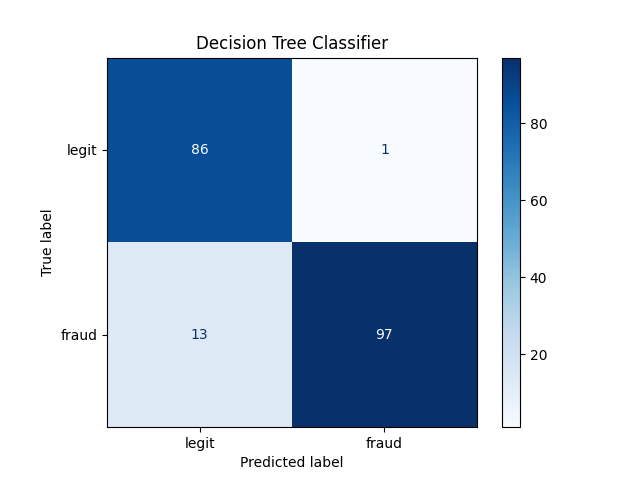
\includegraphics{dt_classifier.png}
    \caption{Confusion matrix for decision tree classifier.}
  \end{figure}
\end{center}

\begin{center}
  \begin{figure}[H]
    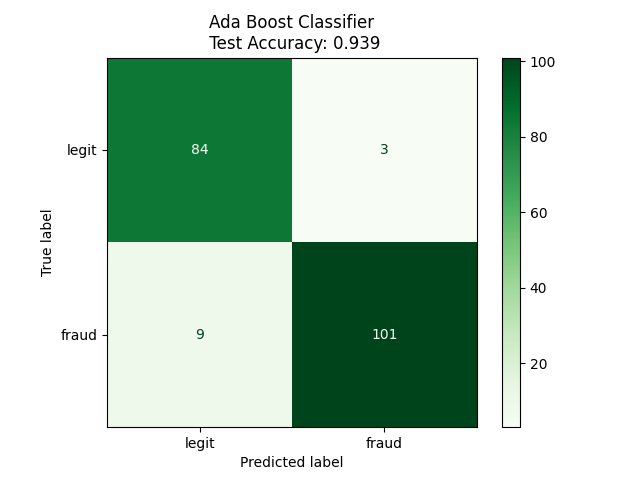
\includegraphics{boost_classifier.png}
    \caption{Confusion matrix for ada boost classifier.}
  \end{figure}
\end{center}

\begin{center}
  \begin{figure}[H]
    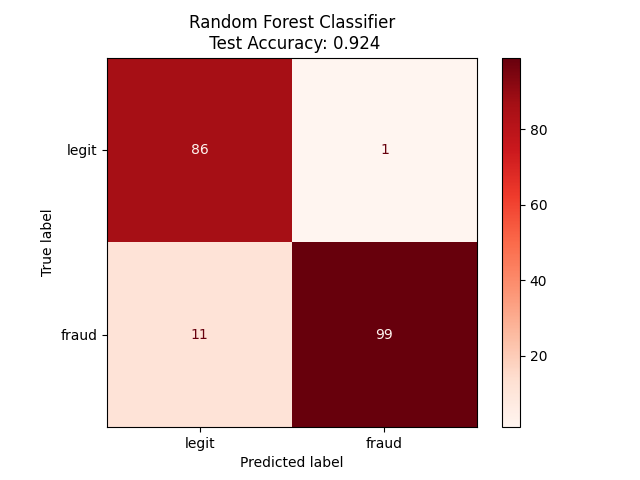
\includegraphics{rf_classifier.png}
    \caption{Confusion matrix for random forest classifier.}
  \end{figure}
\end{center}

\noindent\rule{\textwidth}{0.4pt}\\

\begin{comment}
  \begin{center} 
  \begin{tabular}{|c|c|c|} 
    \hline Stump Number (\%) & Training Accuracy (\%) \\ 
    \hline 
    1 & 16.32\\ 
    2 & 15.91 \\
    3 & 14.25 \\
    4 & 13.56 \\ 
    5 & 14.05  \\ 
    \hline
  \end{tabular}
\end{center}
\end{comment}

\begin{comment}
\subsection*{Solution 7}
\noindent\rule{\textwidth}{0.4pt}\\

\begin{figure}
  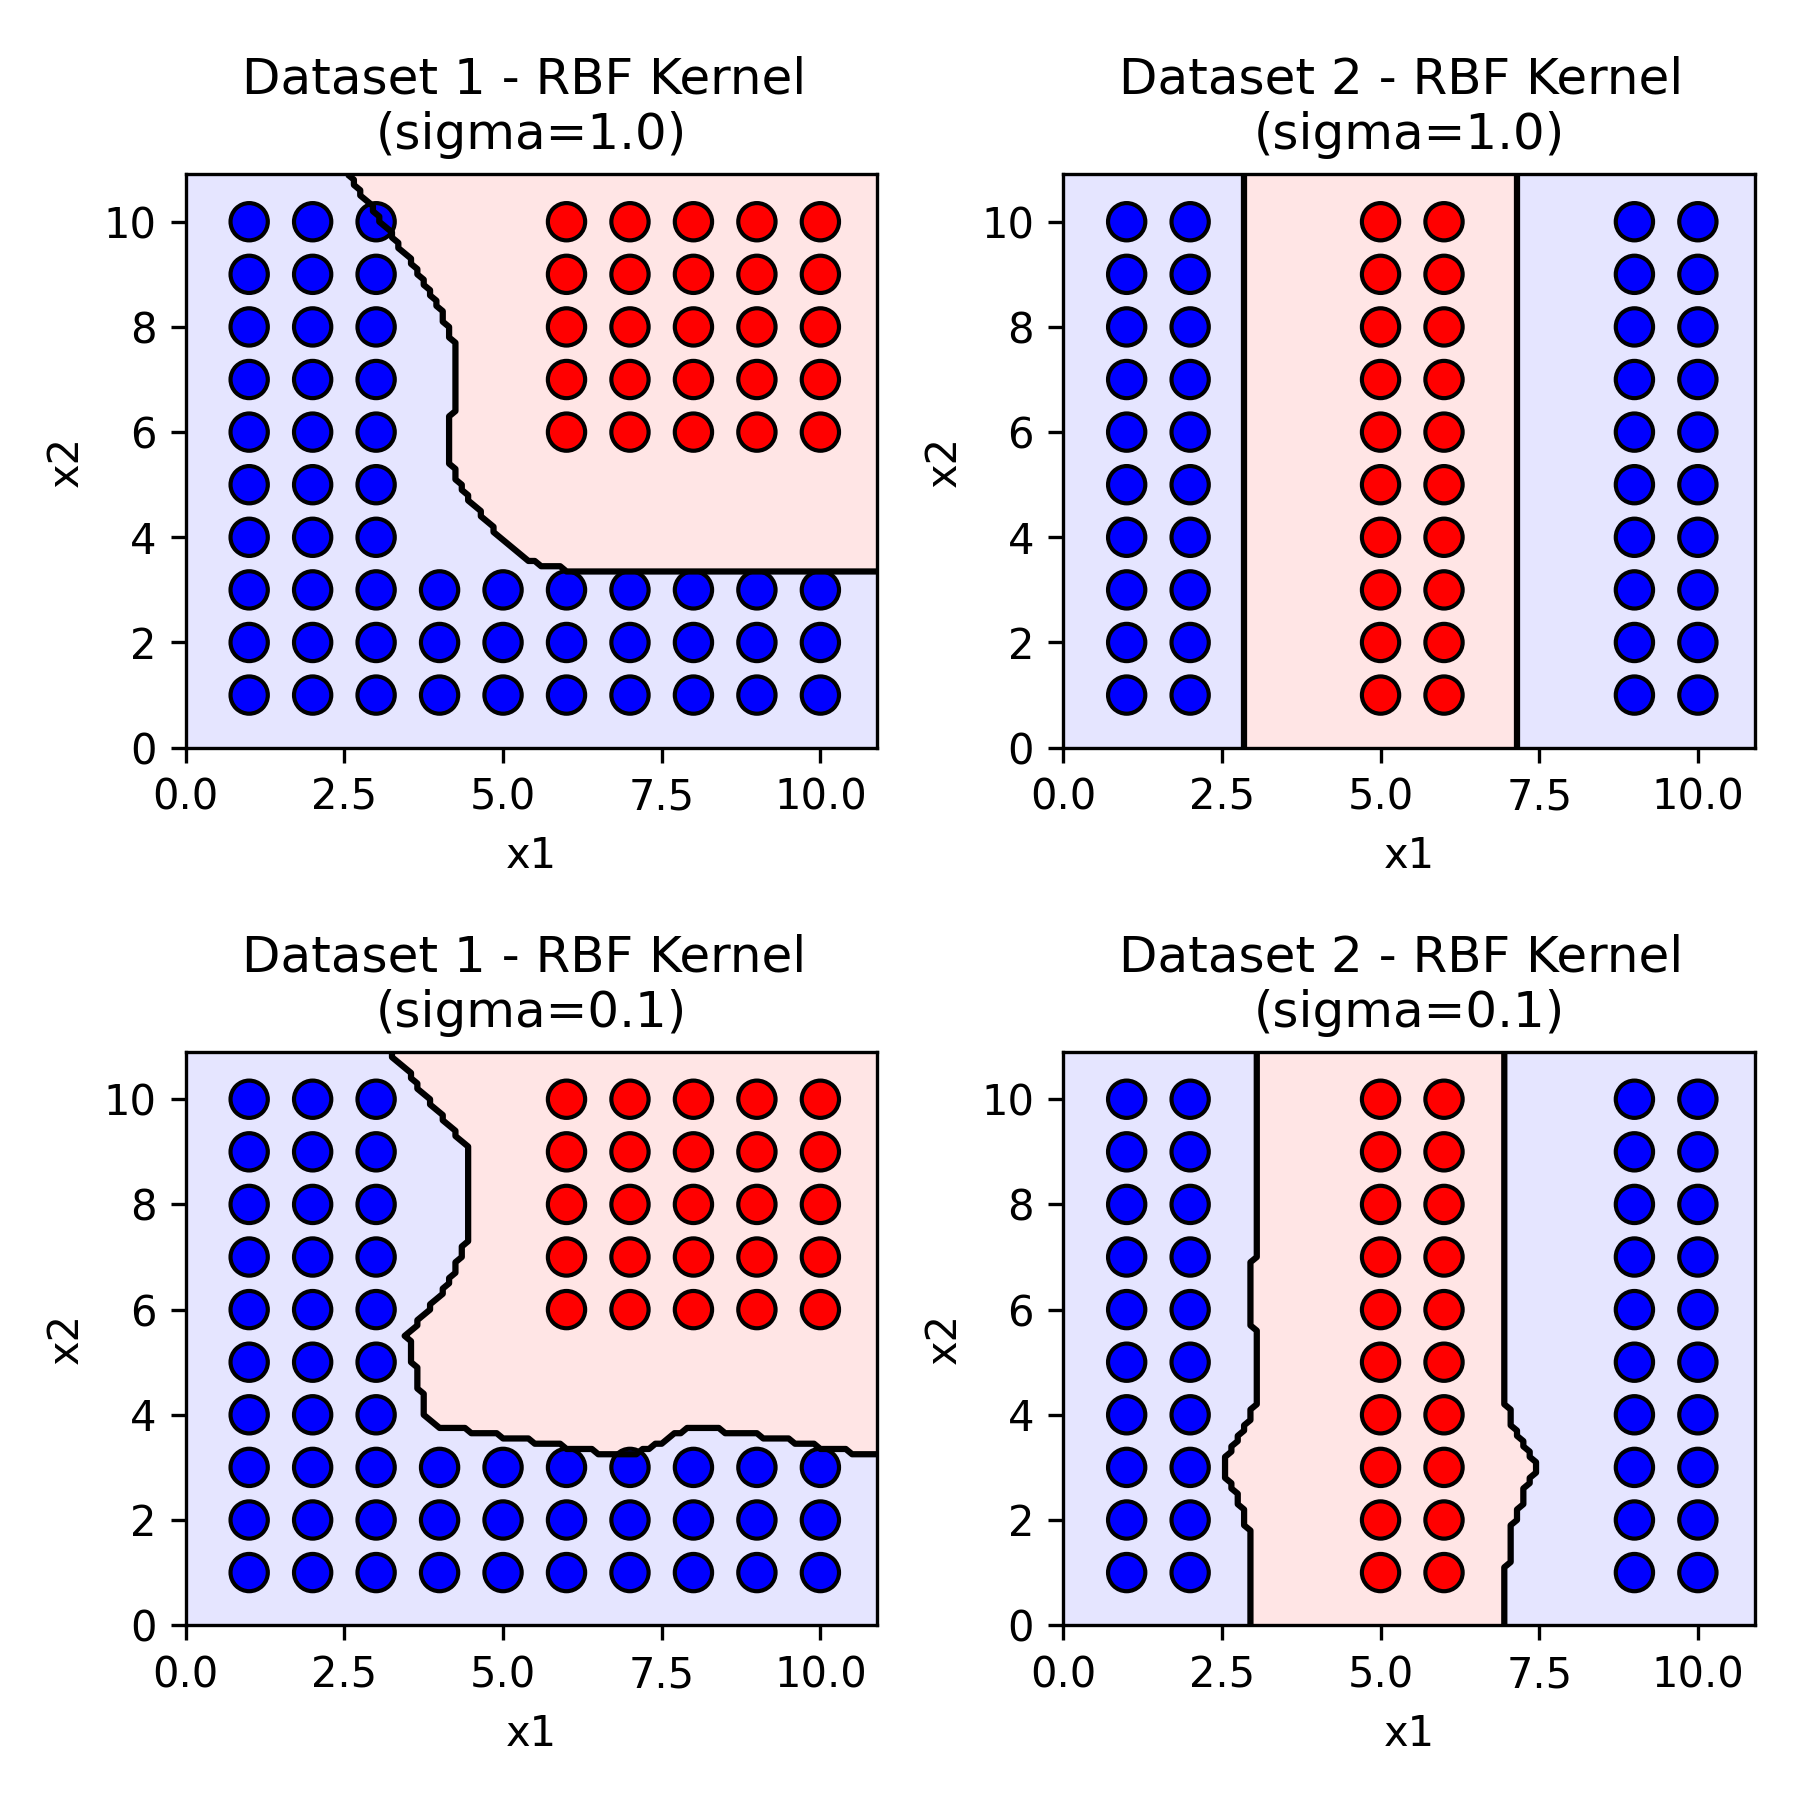
\includegraphics{part_b_rbf_kernel.png}
  \caption{Decision boundary for rbf kernel}
\end{figure}
\noindent\rule{\textwidth}{0.4pt}\\

\subsubsection*{Linear SVM}

\begin{center} 
  \begin{tabular}{|c|c|c|} 
    \hline C Value & Training Error (\%) & Test Error (\%) \\ 
    \hline 
    0.01 & 16.32 & 15.48\\ 
    0.1 & 15.91 & 16.36 \\
    1.0 & 14.25 & 14.04 \\
    10.0 & 13.56 & 13.16 \\ 
    100.0 & 14.05 & 14.78 \\ 
    \hline
  \end{tabular}
\end{center}
\parbox{\textwidth}{Based on the results above it seems that the data is linearly separable.}
\subsubsection*{Quadardic SVM}
\begin{center} 
  \begin{tabular}{|c|c|c|} 
    \hline Training Error (\%) & Test Error (\%)  & Support Vectors\\ 
    \hline 
    0.17 & 2.13 & 17906\\ 
    \hline
  \end{tabular}
\end{center}

\begin{lstlisting}
PYTHON CODE HERE
\end{lstlisting}
\end{comment}
\end{document}

